\documentclass{beamer}

\usepackage[utf8]{inputenc}
\usepackage{color}
\usepackage{xcolor}
\usepackage{amsmath}
\usepackage{amsthm}
\usepackage{amssymb}
\usepackage{graphicx} 
\usepackage{svg}
\usepackage{tikz}
\usepackage{hyperref}

%%% dont split footnotes
\interfootnotelinepenalty=10000

\usepackage{mathtools}

%%% side by side figures
\usepackage{subcaption}

%%% multicols 
\usepackage{multicol}


%tikz
\usepackage{tikz-3dplot}
\usetikzlibrary{arrows.meta}
\usetikzlibrary{external}
\tikzexternalize[prefix=./]

% \usetheme{Madrid}
\usecolortheme{seahorse}
\colorlet{beamer@blendedblue}{teal}
\setbeamertemplate{navigation symbols}{}%remove navigation symbols

\title{Rotations}
\author{Wojciech Pachowiak}
\date{}
%%%%%%%%%%%%%%%%%%%%%%%%%%%%%%%%%%%%%%%%

\newcommand{\aatuple}[4]{(\degree{#1},[#2,#3,#4])}

\newcommand{\aavec}[3]{[#1,#2,#3]}


\newcommand{\hl}[1]{\colorbox{gray!30!white}{\it{#1}}}

%%%%%%%%%%%%%%%%%%%%%%%%%%%%%%%%%%%%%%%%
% sets

\newcommand{\sthree}{\mathbb{S}^3}

\newcommand{\stwo}{\mathbb{S}^2}

\newcommand{\sone}{\mathbb{S}^1}

\newcommand{\sutwo}{\mathbb{SU}(2)}

\newcommand{\sothree}{\mathbb{SO}(3)}
\newcommand{\sotwo}{\mathbb{SO}(2)}

\newcommand{\R}{\mathbb{R}}

\newcommand{\Z}{\mathbb{Z}}

%%%%%%%%%%%%%%%%%%%%%%%%%%%%%%%%%%%%%%
% SHORTCUTS

\newcommand{\selfref}{thesis}

\newcommand{\CS}{CS}

\newcommand{\mX}{\mathbf{R}_X}
\newcommand{\mY}{\mathbf{R}_Y}
\newcommand{\mZ}{\mathbf{R}_Z}

%%%%%%%%%%%%%%%%%%%%%%%%%%%%%%%%%%%%%%

\newcommand{\overbar}[1]{\mkern 1.5mu\overline{\mkern-1.5mu#1\mkern-1.5mu}\mkern 1.5mu}


\newcommand{\trace}{\text{Tr}}

\newcommand{\degree}[1]{{#1}^{\circ}}

\newcommand{\rotaxisn}{\rotaxis{n}}

\newcommand{\rotaxis}[1]{\mathbf{#1}}

\newcommand{\lrotaxis}[1]{\mathbf{\lowercase{#1}}}
\newcommand{\grotaxis}[1]{\mathbf{\uppercase{#1}}}


\newcommand{\rotmat}[2]{\mathbf{R}(\rotaxis{#1},#2)}
\newcommand{\trotmat}[2]{\mathbf{R}^\top(\rotaxis{#1},#2) }


\newcommand{\rotmatII}[1]{
	\begin{bmatrix}
		\cos{#1} & -\sin{#1} \\
		\sin{#1} & \cos{#1}
	\end{bmatrix}
}

\newcommand{\complexnumb}[2]{
#1 + i#2
}

\newcommand{\vecsymb}[1]{{\mathbf{\lowercase{#1}}}}
\newcommand{\vv}[1]{{\mathbf{\lowercase{#1}}}}

\newcommand{\vecthree}[3]{
\begin{bmatrix}
	#1 &
	#2&
	#3
\end{bmatrix}}

\newcommand{\vecthreecol}[3]{
	\begin{bmatrix}
		#1 \\
		#2\\
		#3
\end{bmatrix}}

\newcommand{\vectwocol}[2]{
	\begin{bmatrix}
		#1 \\
		#2
\end{bmatrix}}

\newcommand{\tvectwocol}[2]{
	\begin{bmatrix}
		#1 &
		#2
\end{bmatrix}^\top}

\newcommand{\tvecthree}[3]{
\vecthree{#1}{#2}{#3}^\top	
}

\newcommand{\sphercoordsvec}{
	\tvecthree{\cos\alpha\sin\beta}{\sin\alpha\sin\beta}{\cos\beta}
}

\newcommand{\genmat}[1]{\mathbf{R}_{#1}}

\newcommand{\tgenmat}[1]{\mathbf{R}_{#1}^\top}


\newcommand{\pihalf}{\frac{\pi}{2}}


\newcommand{\norm}[1]{\left\lVert#1\right\rVert}

\newcommand{\interpolate}[1]{\twoheadrightarrow_{#1}}

\newcommand{\crossmat}[1]{\left[#1\right]_{\times}}

\newcommand{\crossmatfull}[3]{
\begin{bmatrix}
	0 & -#3 & #2 \\
	#3 & 0 & -#1 \\
	-#2 & #1 & 0 
\end{bmatrix}
}

%%%%%%%%%%%%%%%%%%%%%%%%%%%%%%%%%%%
% quaternions

\newcommand{\quattw}[2]{
	t_#2(#1)
}

\newcommand{\quatsw}[3]{
	s_#3(#1, #2)
}

\newcommand{\quat}[4]{
	\textstyle(#1,(#2,#3,#4))
}

\newcommand{\quatvec}[2]{
	\textstyle \left(#1, \mathbf{#2}\right)
}

\newcommand{\quatvecmanual}[2]{
	\textstyle(#1, #2)
}

\newcommand{\quatrotaxis}[2]{
\textstyle q(\rotaxis{#1},#2)
}


\newcommand{\quatrotaxisinv}[2]{
	\textstyle q^{-1}(\rotaxis{#1},#2)
}

\newcommand{\quataa}[2]{
\quatvecmanual{\cos\frac{#2}{2}}{\rotaxis{#1}\sin\frac{#2}{2}}
}

\newcommand{\idmat}{\mathbf{I}}

%%%%%%%%%%%%%%%%%%%%%%%%%%%%%%%%%%%%
% eulers 

\newcommand{\eulangovals}[3]{(\degree{#1},\degree{#2},\degree{#3})}


\begin{document}

\frame{\titlepage}

\AtBeginSection[]
{
  \begin{frame}
    \frametitle{Table of Contents}
    \tableofcontents[currentsection]
  \end{frame}
}

%##################################################################################


\section{Convetions}

\begin{frame}
\frametitle{Coordinate systems}
What orientations do the following mathematical rotation representations express?
\begin{itemize}
    \item Euler angles $\eulangovals{41}{-18}{-83}$ in XYZ extrinsic order
    \item Quaternion $\quat{0.73}{0.16}{-0.34}{-0.57}$
    \item Axis angle tuple $\aatuple{86}{0.24}{-0.5}{-0.84}$
    \item Axis angle vector $\aavec{0.36}{-0.75}{-1.26}$
    \item 3D rotation matrix 
    $$        
        \begin{bmatrix}
            0.116 & 0.725 & -0.68 \\
            -0.944 & 0.3 & 0.15 \\
            0.31 & 0.624 & 0.718
        \end{bmatrix}
    $$
\end{itemize} 
The same orientation but with respect to what coordinate system (frame of reference)?
\end{frame}

\begin{frame}
\frametitle{Active and passive rotations}
Which is moving? Objects within a coordinate system or the coordinate system itself?

\begin{figure}
	\centering
	\def\sqlen{0.2}
	\def\sqshift{0.5}
	\def\axlen{0.5}
	\def\ang{20}
	\def\arr{0.282842712}
	
	\begin{subfigure}{0.45\textwidth}
		\centering
		\begin{tikzpicture}[thick,scale=5]
			
			\draw[-Stealth, black!25] (0,0) -- (0,\axlen);
			\draw[-Stealth, black!25] (0,0) -- (\axlen,0);
			
			\draw[red,-Stealth] (\arr,0) arc (0:\ang:\arr) node[right=4mm, below=0mm]{$\theta$};
			
			\draw[-Stealth, rotate=\ang] (0,0) -- (0,\axlen);
			\draw[-Stealth, rotate=\ang] (0,0) -- (\axlen,0);
			
			\draw[black] 
			(\sqlen,\sqlen) -- (\sqlen,-\sqlen) -- (-\sqlen,-\sqlen) -- (-\sqlen,\sqlen) -- (\sqlen,\sqlen); 
			
			
		\end{tikzpicture}
		%	\includesvg[scale=0.5]{"./svg/passive_rotation.svg"}
		%	\includegraphics[width=\linewidth]{passive_rotation.png}
		\caption{Passive rotation}
	\end{subfigure}
	\hfill
	\begin{subfigure}{0.45\textwidth}
		\centering
		
		\begin{tikzpicture}[thick,scale=5]
			\draw[-Stealth, black] (0,0) -- (0,\axlen);
			\draw[-Stealth, black] (0,0) -- (\axlen,0);
			
			\draw[black!25, rotate=0] 
			(\sqlen,\sqlen) -- (\sqlen,-\sqlen) -- (-\sqlen,-\sqlen) -- (-\sqlen,\sqlen) -- (\sqlen,\sqlen); 
			
			\draw[red,-Stealth] ({cos(45)*\arr},{sin(45)*\arr}) arc (45:45-\ang:\arr) node[right=2mm, above=2mm]{$-\theta$};
			
			\draw[black, rotate=-\ang] 
			(\sqlen,\sqlen) -- (\sqlen,-\sqlen) -- (-\sqlen,-\sqlen) -- (-\sqlen,\sqlen) -- (\sqlen,\sqlen); 
			
		\end{tikzpicture}
		
		%	\includesvg[scale=0.5]{"./svg/active_rotation.svg"}
		%	\includegraphics[width=\linewidth]{active_rotation.png}
		\caption{Active rotation}
	\end{subfigure}
\end{figure}

To convert between these two perspectives, invert the rotation:
$$
\mathbf{R}_{active} = \mathbf{R}^{-1}_{passive}
$$

\end{frame}


\begin{frame}
\frametitle{Handedness of coordinate system}
\begin{figure}
    \centering
    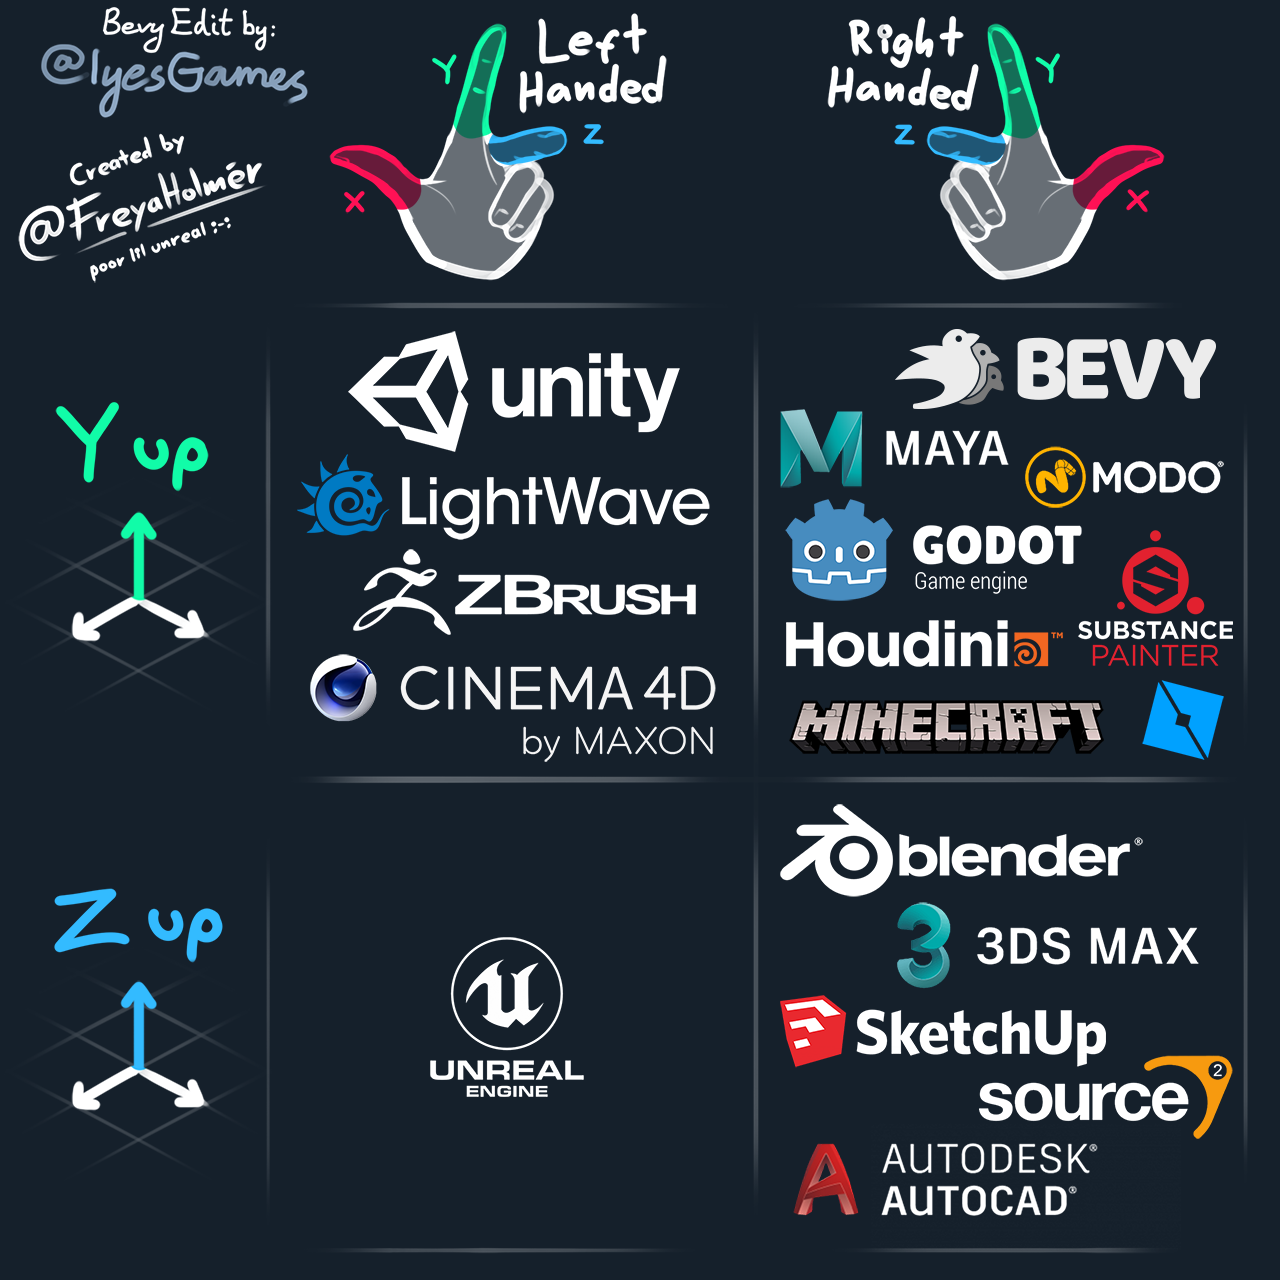
\includegraphics[width=0.8\textheight]{assets/3D_soft_handedness.png}
	\caption*{\url{https://bevy-cheatbook.github.io/fundamentals/coords.html}}
\end{figure}
\end{frame}

\begin{frame}
\frametitle{Positive angle}
Is positive angle clockwise or counterclockwise when looking along some axis?
\begin{figure}
    \centering
    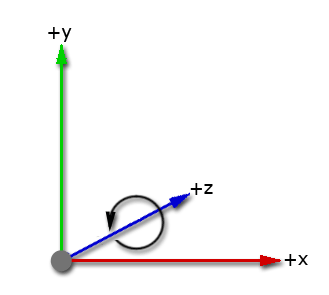
\includegraphics[width=0.7\textheight]{assets/unity-axis-with-rotation_positive_angle.png}
	\caption*{\url{https://docs.unity3d.com/Manual/QuaternionAndEulerRotationsInUnity.html}}
\end{figure}
\end{frame}

\begin{frame}
\frametitle{Forward, up, right vectors}
Which vectors are considered forward, upward, rightward, leftward, etc.?
\begin{figure}
    \centering
    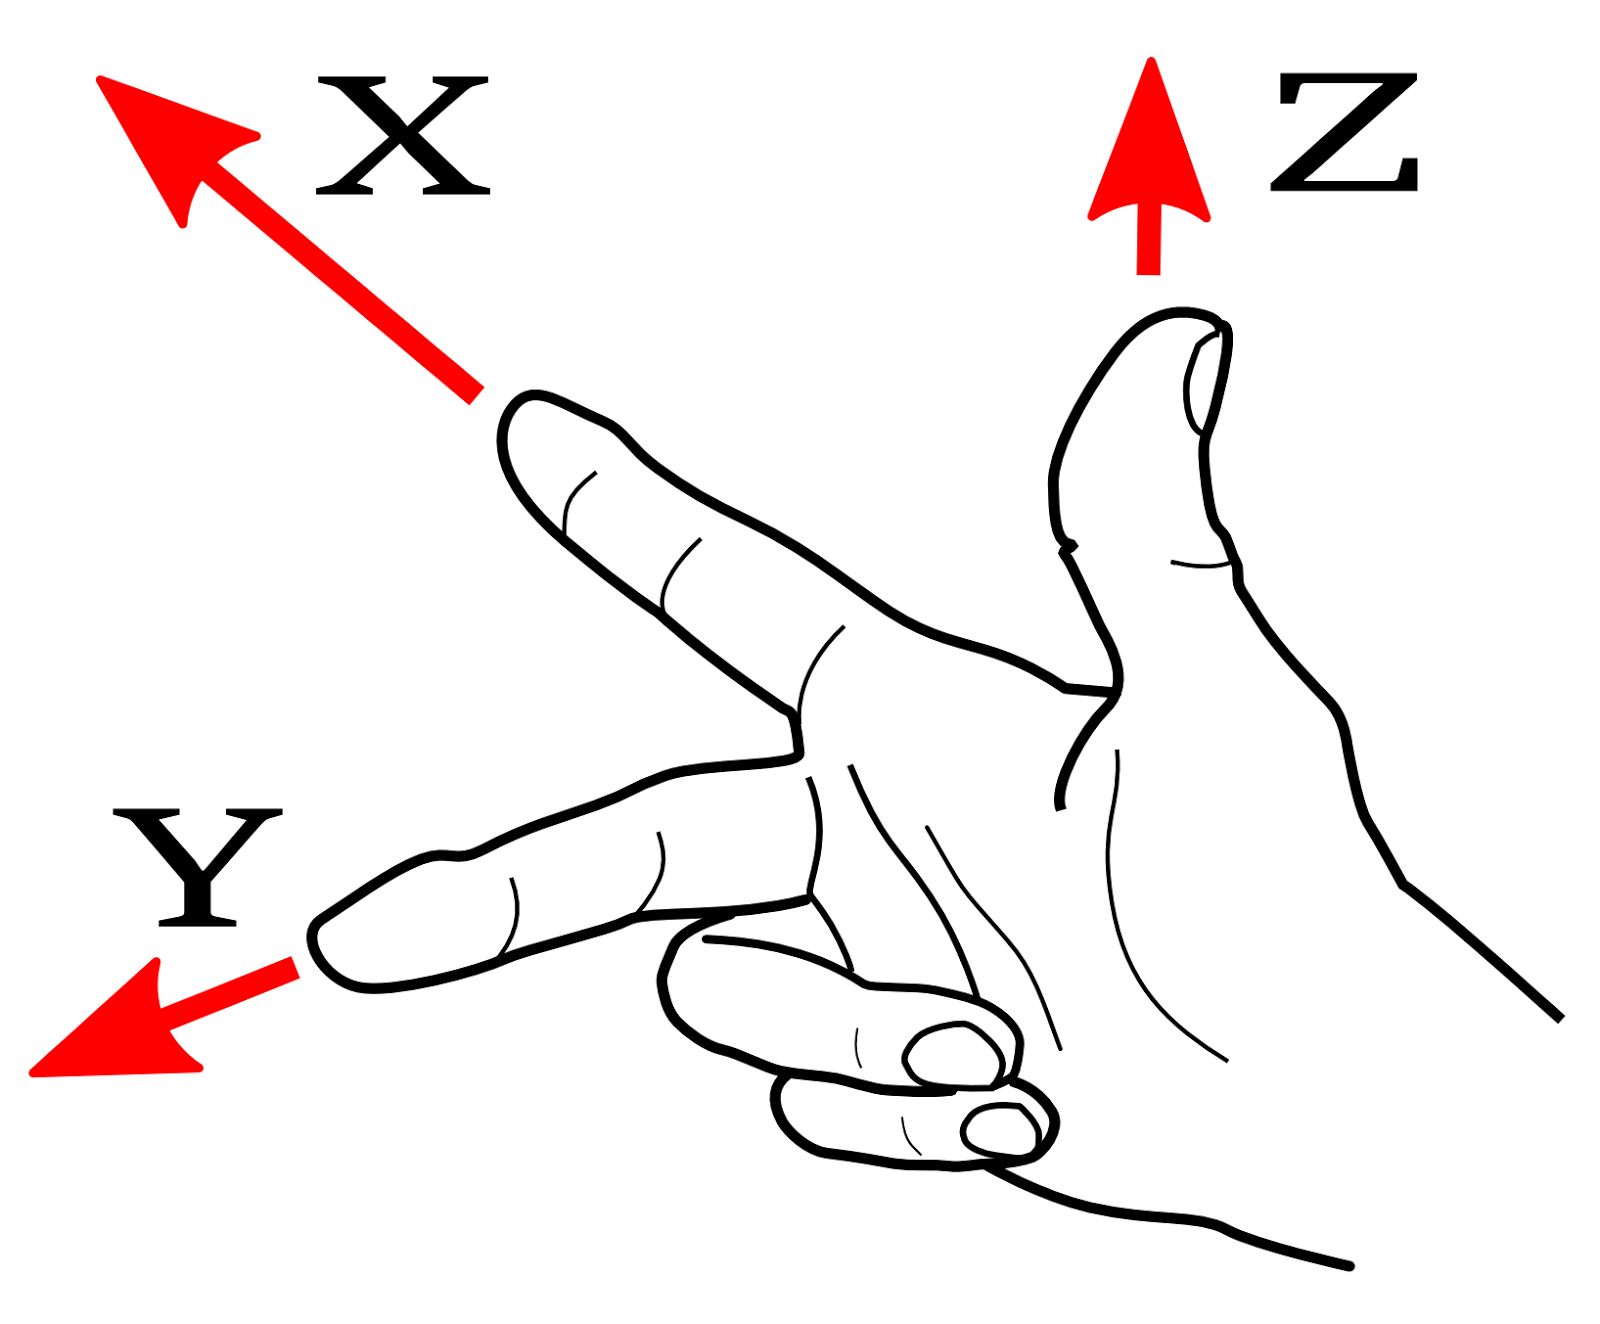
\includegraphics[width=0.8\textheight]{assets/fingers.png}
	\caption*{\url{https://stackoverflow.com/a/34068511}}
\end{figure}
\end{frame}

\begin{frame}
\frametitle{Intrinsic and extrinsic rotations}
When it comes to Euler angles, are rotations performed around the global axes or some local axes?

TODO formula for conversion between them
\vfill 	
See the pictures for a visual explanation:
\url{https://en.wikipedia.org/w/index.php?title=Davenport_chained_rotations&oldid=1222677779\#Conversion_between_intrinsic_and_extrinsic_rotations}
\end{frame}
        
%##################################################################################

\section{Mathemtical representations}


\begin{frame}
\frametitle{2D rotations}
\end{frame}


\begin{frame}
\frametitle{Euler angles}
\end{frame}


\begin{frame}
\frametitle{3D rotation matrices: Euler-angle-like}
\end{frame}


\begin{frame}
\frametitle{3D rotation matrices: axis-angle-like}
\end{frame}


\begin{frame}
\frametitle{Quaternions}
\end{frame}


\begin{frame}
\frametitle{Rodriguez formula}
\end{frame}
    
    

\begin{frame}
\frametitle{Axis-angle, exponential map}
\end{frame}
    

\begin{frame}
\frametitle{In SciPy}
\url{https://docs.scipy.org/doc/scipy/reference/generated/scipy.spatial.transform.Rotation.as_quat.html}
\vfill
Note the \hl{seq} argument in \hl{as\_euler} method. Also note the \hl{canonical} and \hl{scalar\_first} arguments in \hl{as\_quat}.
\vfill
We didn't cover: 
\begin{itemize}
	\item Davenport angles --- like Euler angles but generalized to nonperpendicular axes.  
	\item Modified Rodriguez Parameters (MRP) --- like axis-angle vectors but the angle of rotation is transformed.
\end{itemize}
\end{frame}

%##################################################################################

\section{Miscellaneous}


\begin{frame}
\frametitle{Gimbal lock}
\end{frame}


\begin{frame}
\frametitle{A-to-B rotation interpolation}
\end{frame}


\begin{frame}
\frametitle{A-to-C-through-B rotation interpolation}
\end{frame}



%##################################################################################

\end{document}

%##################################################################################
